
% linear svm (test) prediction map
\begin{figure}[H]
    \centering
    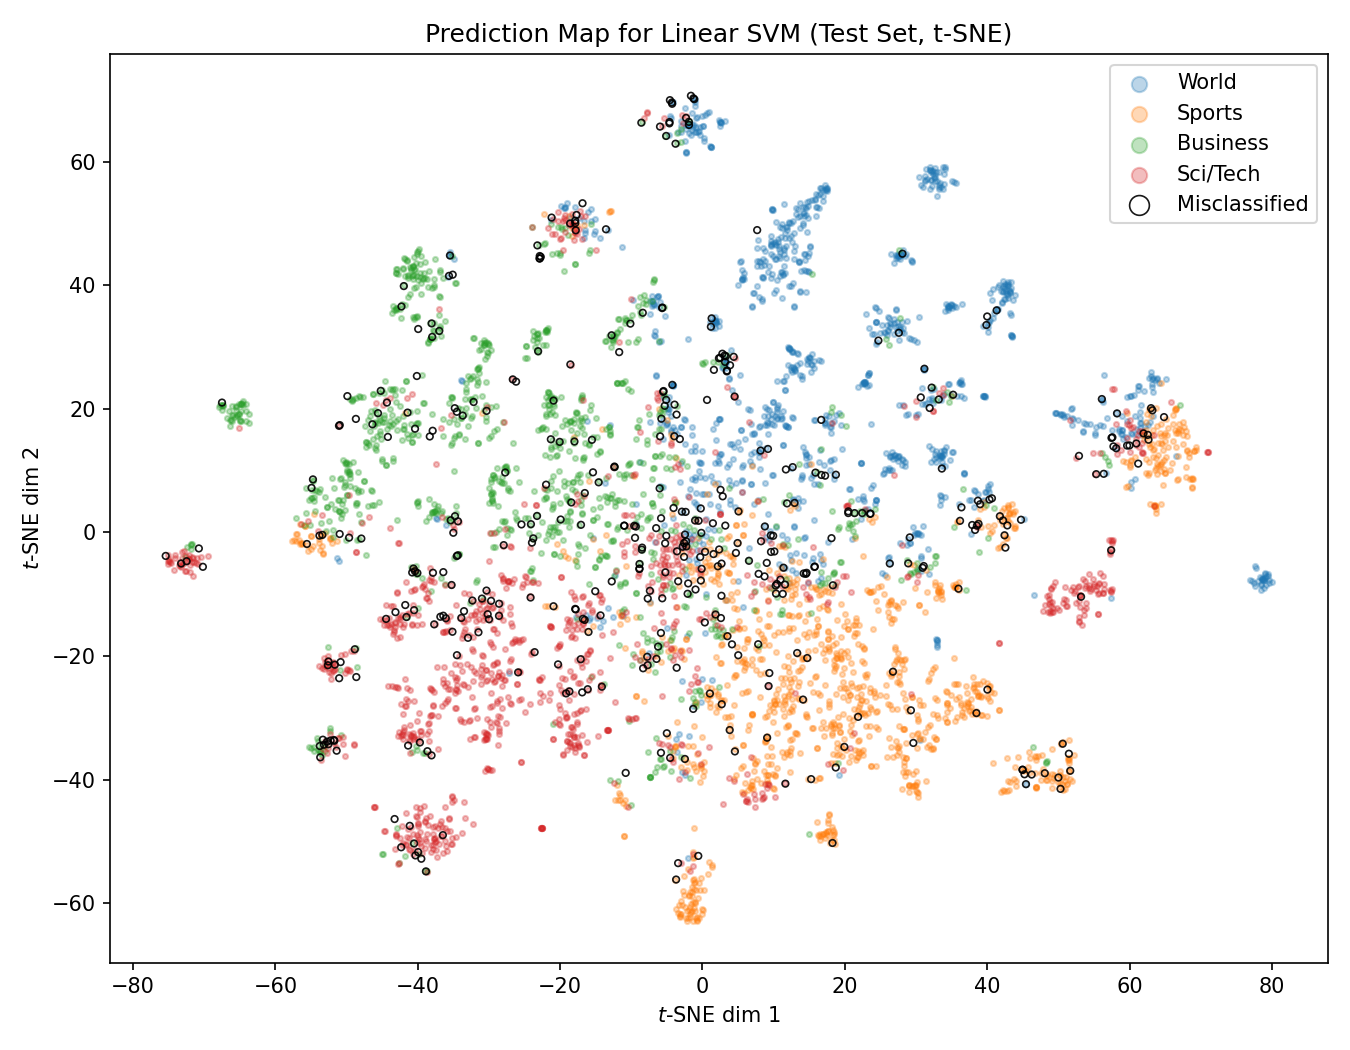
\includegraphics[width=0.5\textwidth]{../figures/linear_svm_test_prediction_map.png}
    \caption{t-SNE Projection of Linear SVM Predictions on Test Set}
\end{figure}

% logistic regression (test) prediction map
\begin{figure}[H]
    \centering
    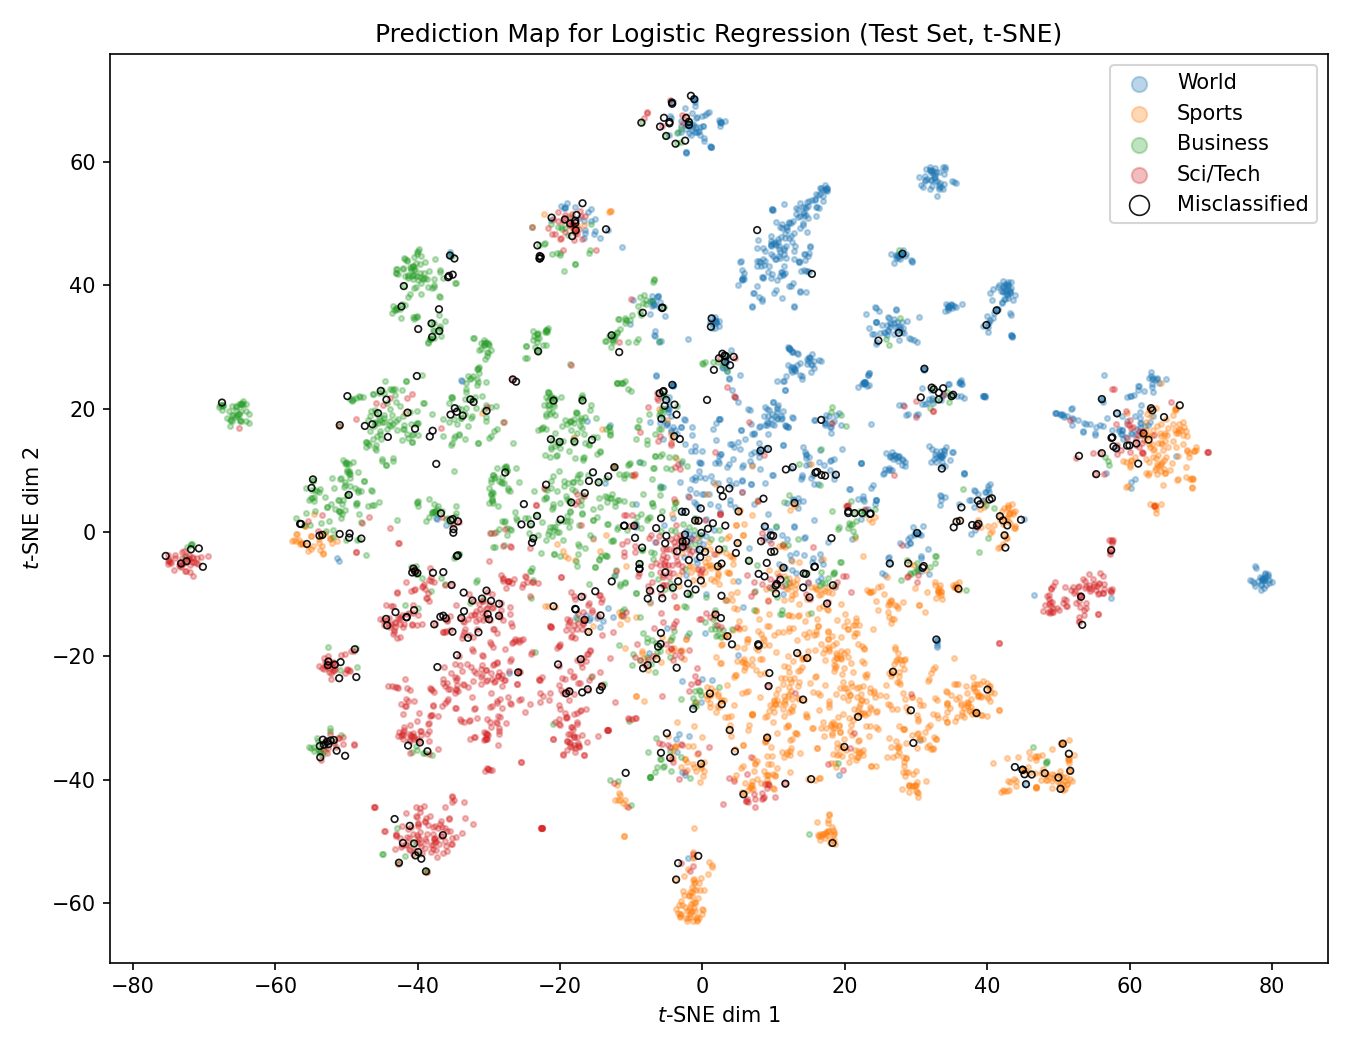
\includegraphics[width=0.5\textwidth]{../figures/logistic_regression_test_prediction_map.png}
    \caption{t-SNE Projection of Logistic Regression Predictions on Test Set}
\end{figure}

% speak about the overlapping clusters in the t-SNE projection, and how they relate to the confusion matrix (e.g., which classes are most often confused, and how that is reflected in the projection)

% mention that sci/tech gets confused with business, and that this is reflected in the t-SNE projection where the clusters for these classes overlap more than the others

% find examples of sci/tech mislabeled as business, and analyze them to see if there are any common features that might explain the confusion (e.g., certain keywords that are common in both classes)

% also mention that the confusion between these classes is not surprising given that they can both contain articles about technology companies, which might have similar language and keywords (e.g., "Apple", "Google", "Microsoft" could appear in both classes)